% Intended LaTeX compiler: xelatex
\documentclass[a4paper, 12pt]{article}
\usepackage{graphicx}
\usepackage{grffile}
\usepackage{longtable}
\usepackage{wrapfig}
\usepackage{rotating}
\usepackage[normalem]{ulem}
\usepackage{amsmath}
\usepackage{textcomp}
\usepackage{amssymb}
\usepackage{capt-of}
\usepackage{hyperref}
\usepackage[danish]{babel}
\usepackage{mathtools}
\usepackage[margin=3.0cm]{geometry}
\hypersetup{colorlinks, linkcolor=black, urlcolor=blue}
\setlength{\parindent}{0em}
\parskip 1.5ex
\author{Matematik A}
\date{Vibenhus Gymnasium}
\title{Vektorfunktioner\\\medskip
\large Gamle eksamensopgaver}
\hypersetup{
 pdfauthor={Matematik A},
 pdftitle={Vektorfunktioner},
 pdfkeywords={},
 pdfsubject={},
 pdfcreator={Emacs 27.2 (Org mode 9.4.4)}, 
 pdflang={Danish}}
\begin{document}

\maketitle


\section*{Gamle eksamensopgaver om vektorfunktioner}
\label{sec:org1d8085f}

På de følgende sider vil I finde en række af gamle eksamensopgaver omhandlende vektorfunktioner. Jeg forventer \emph{ikke}, at I skal nå at gennemarbejde alle opgaverne. Det jeg til gengæld forventer af jer, er at I skriver opgavebesvarelserne ind på computer, med fyldestgørende forklaringer, mellemregninger og grafer. \textbf{Fokus er altså dels på at løse opgaven, og dels at skabe fortrolighed med formeleditor og geogebra/CAS.}

\begin{itemize}
\item I skal arbejde sammen i makkerpar og makkerskabsgrupper. Et makkerpar vælger én af opgaverne og det andet makkerpar vælger en anden af opgaverne.
\item Hvert makkerpar udarbejder en skriftlig løsning til deres opgave, som beskrevet tidligere.
\item Efter endt løsning, skal makkerparrene \textbf{\textbf{mundtligt}} præsentere deres løsninger for hinanden i makkerskabsgrupperne.
\end{itemize}

\begin{center}
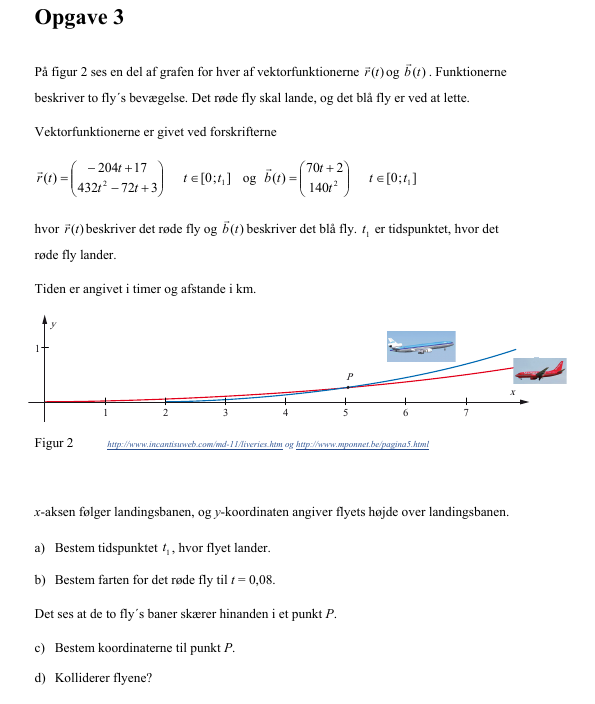
\includegraphics[width=.9\linewidth]{img/opg1.png}
\end{center}
\begin{center}
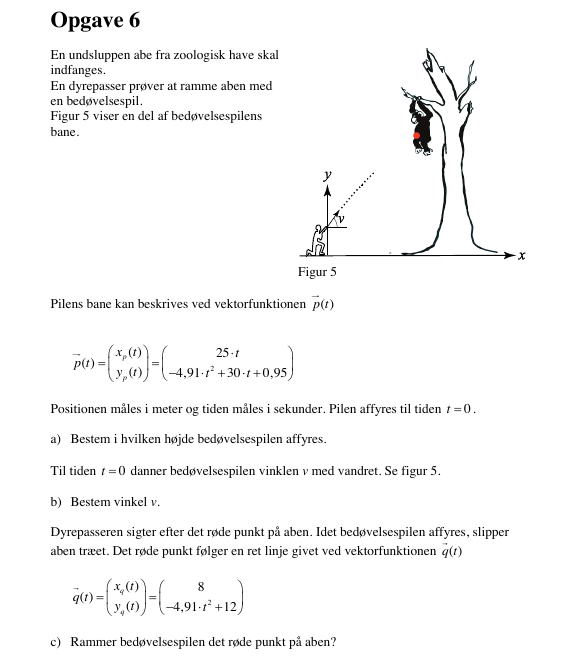
\includegraphics[width=.9\linewidth]{img/opg2.png}
\end{center}
\begin{center}
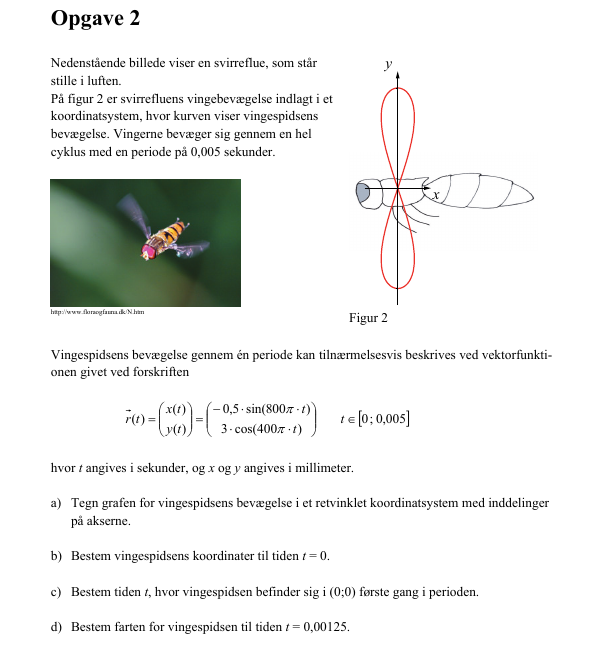
\includegraphics[width=.9\linewidth]{img/opg3.png}
\end{center}
\begin{center}
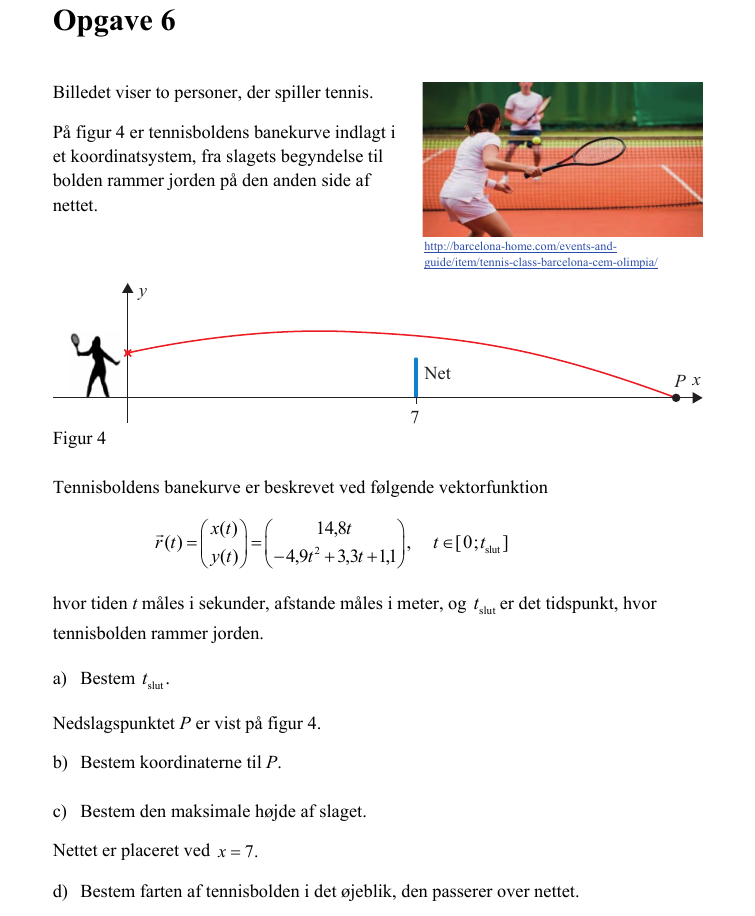
\includegraphics[width=.9\linewidth]{img/opg4.png}
\end{center}
\begin{center}
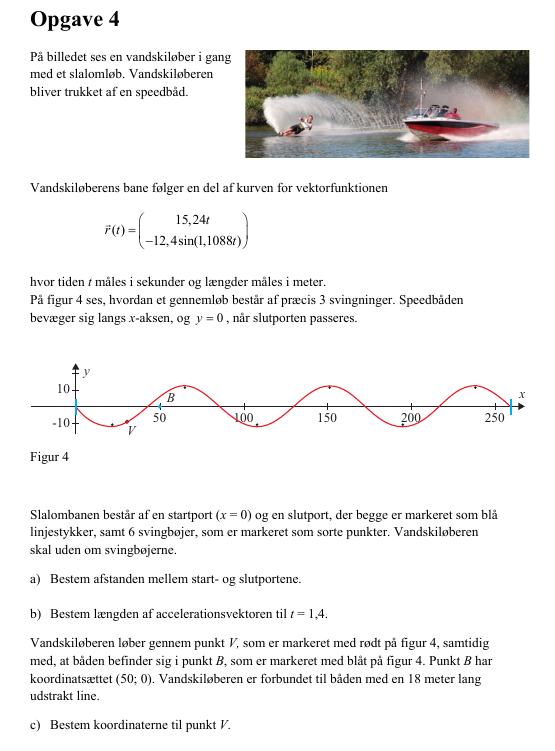
\includegraphics[width=.9\linewidth]{img/opg5.png}
\end{center}


\newpage
\section*{Formelsamling til vektorfunktioner}
\label{sec:org1f9e214}

Jeres sidste opgave er, at skrive jeres egen formelsamling til vektorfunktioner.

I kan formelsamlingen fra matematikbogen her: \url{https://mathtxa.systime.dk/?id=p386}, og lade jer inspirere af den.

Det vigtigste er dog, \textbf{at I selv skriver det hele ind. Formlerne skal skrives i en formeleditor og teksten skal I også selv skrive. Ikke noget med at copy-paste eller tager screenshots.}

Pointen med denne opgave er, at I får set alle formlerne og får bearbejdet dem ved selv at skrive dem ind.
\end{document}